\subsubsection{GTFS - Probleme und Herausforderungen}
\label{ssub:gtfs_probleme_und_herausforderungen}
   Bereits 1993 stellte \texttt{Jakob Nielsen} einen Richtwert für die Antwortzeit einer schnellen Webanwendung vor:

  \begin{quote}
    \textit{"`1.0 second is about the limit for the user's flow of thought to stay uninterrupted, even though the user will notice the delay. Normally, no special feedback is necessary during delays of more than 0.1 but less than 1.0 second, but the user does lose the feeling of operating directly on the data."'}\parencite{nielsen}
  \end{quote}

  Ob oder wie dies Antwortzeit erreicht werden kann, soll hier nicht vertieft werden, denn zu diesem Thema habe ich bereits meine Bachelorarbeit gewidmet\parencite{lorer}.

  Damit eine Webanwendung aber überhaupt eine Chance hat, diese Geschwindigkeitsmarke zu erreichen, ist eine schnelle Antwortzeit des Backends sehr wichtig. Dabei sind Antwortzeiten Innerhalb von 0 bis 200 Millisekunden ein sehr guter Wert. Natürlich gilt: Je weniger umso besser. Diese Benchmark mit dem GTFS Format zu erreichen war eine der Hauptherausforderungen dieser Arbeit.\\

  Das GTFS Format hat den entscheidenden Nachteil, dass es eine hohe Komplexität aufweist, sobald Daten aus verschiedenen Tabellen benötigt werden. Für eine Live Visualisierung, sind Daten aus nahezu allen Tabellen relevant. Abbildung~\ref{fig:gtfs_joined_tables} zeigt, welche davon benötigt - beziehungsweise nicht benötigt werden (grau).

  \begin{figure}[ht]
    \begin{center}
      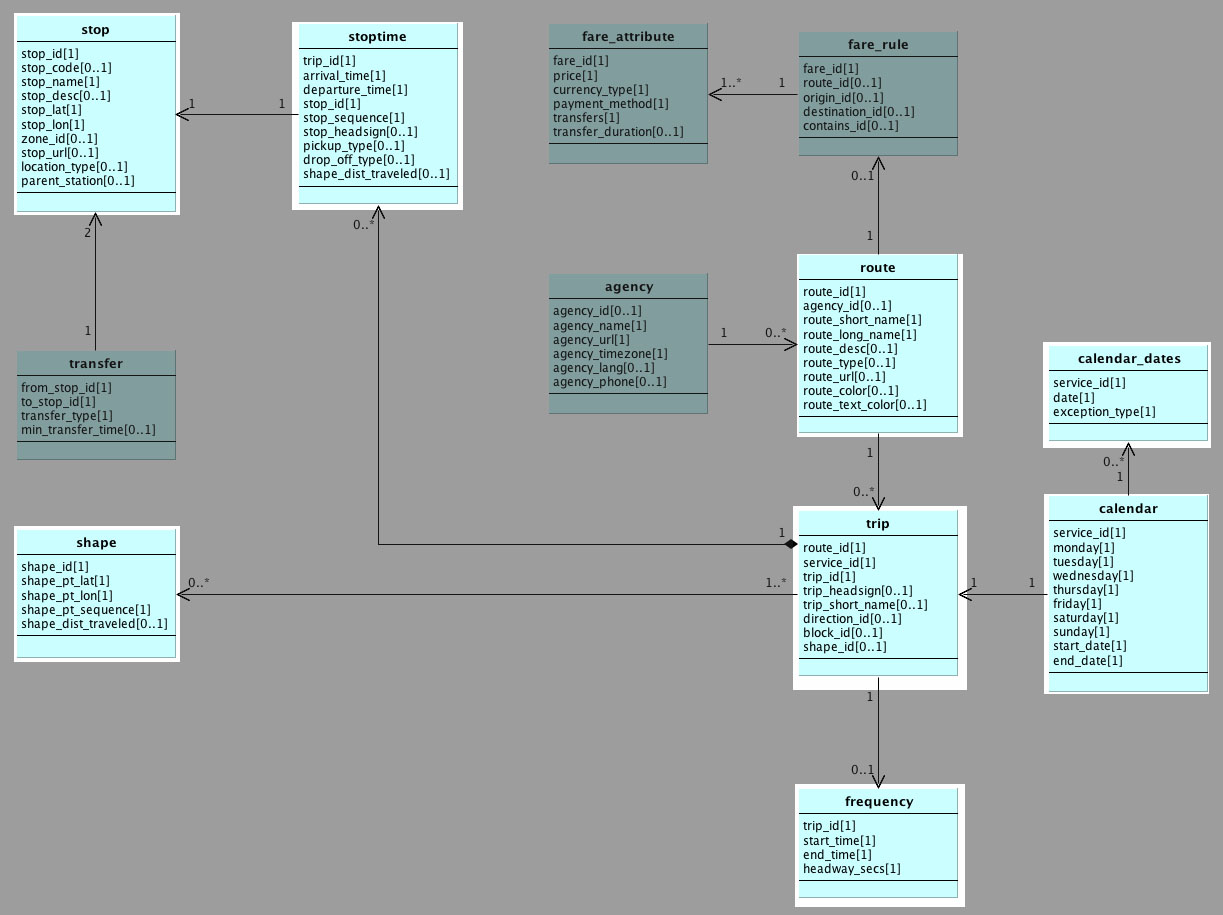
\includegraphics[width=\textwidth]{gtfs_joined_tables.jpg}
      \caption{Benötigte GTFS Tabellen\parencite{google_gtfs_reference}}
      \label{fig:gtfs_joined_tables}
    \end{center}
  \end{figure}

  Das UML Diagramm ist auf den ersten Blick relativ simpel zu verstehen und die Grundlagen der verschiedenen Relationen wurde bereits in Kapitel~\ref{ssec:gtfs_datenformat} beschrieben. Wo liegt also das Problem? In Worten ließe sich diese Datenbankabfrage mit folgendem Statement beschreiben: 

  \begin{quote}
    \label{query_statement}
    \textit{"`Gib uns alle aktiven Trips mit deren Linienverlauf, die am heutigen Tag aktiv sind und in einer Zeitspanne zwischen $t_a$ und $t_b$ liegen."'}
  \end{quote}

  Das große Problem dieses Satze liegt in der Zeitkomponente \textit{"`Trips die am heutigen Tag aktiv sind zwischen ..."'}. Die Trip Tabelle selbst (bezogen auf Abbildung~\ref{fig:gtfs_joined_tables}), hat dies bezüglich keinerlei Informationen darüber. Auch die Calendar- und Calendar-Dates Tabelle beinhaltet nur Informationen, an welchem Datum ein Trip stattfindet, nicht aber um welche Uhrzeit. 

  Erst die Stoptime Tabelle ermöglicht es uns, eine Aussage zu treffen, wann ein Trip aktiv ist. Über die zwei Felder \texttt{arrival\_time} und \texttt{departure\_time} lässt sich sagen, zu welchem Zeitpunkt ein Vehicle an einer Station anhält. Die erste und letzte Station ($S_1$ und $S_n$) geben uns also einen zeitlichen Rahmen, in dem der Trip aktiv ist.
  Hierbei wird klar, dass allein die Beantwortung der Frage zur zeitlichen Komponente, bereits sehr viele Daten aus verschiedenen Tabellen benötigt. Die anderen Tabellen wie \texttt{shape}, \texttt{route}, \texttt{stop} und \texttt{frequency} würden für weitere Informationen wie Vehicle Farbe, Stop Position (Längen- und Breitengrad) oder den Linienverlauf (shape) benötigt werden. Um an die Daten zu gelangen, müssen alle benötigten Tabellen mittels SQL \texttt{JOIN} miteinander verknüpft werden. Dies geschieht durch die Verbindung der einzelnen Reihen zweier Tabellen (TabelleA und TabelleB) gegen eine Verknüpfungsbedingung. Das Resultat ist eine neue Ergebnistabelle mit den Inhalten der kombinierten Reihen. Solche Verknüpfungen sind besonders dann Zeitintensiv, wenn eine große Menge an Daten (siehe Tabelle:~\ref{table:table_metrics}) kombiniert werden. Die Metriken der Tabellen sind dabei wie folgt:

  \begin{longtable}{|>{\raggedright \arraybackslash}p{5.0cm}|>{\raggedright \arraybackslash}p{5.0cm}|>{\raggedright \arraybackslash}p{5.0cm}|}
  \caption{Tabellen Metriken} \label{table:table_metrics}\\
    \hline
    Tabellen Name & Anzahl Reihen\\
    \hline
    trips.txt & 71,000\\
    stop\_times.txt & 1,3000,000\\
    stops.txt & 7,900\\
    shapes.txt & 1,085,860\\
    \hline
  \end{longtable}
  
  Die für das oben genannte Statement~\ref{query_statement} äquivalente SQL-Abfrage ist aufgrund seiner Länge (113 Zeilen Code) im Anhang unter Listing~\ref{lst:get_active_trips_query} zu finden. Diese SQL Abfrage ist allerdings nicht Performant. Sollen alle Trips in einem Zeitraum von 1 - 15 Minuten gefunden werden, sind bereits Rechenzeiten entstanden, die aufgrund ihrer langen Laufzeit abgebrochen werden mussten. In mehreren Iterationen wurde versucht die SQL-Abfrage zu optimieren, was allerdings keine Verbesserung herbeiführte. Es sind zu viele JOIN Verknüpfungen und WHERE Bedingungen in dieser Abfrage, als das sich eine Performante Lösung damit finden lässt. Es musste ein neuer Ansatz gefunden werden um Abfragezeiten erheblich zu verringern.
  
% subsubsection gtfs_probleme_und_herausforderungen (end)